\section{Finger Knuckle Acquisition and Segmentation}

We incorporated an FBI-compliant slap-fingerprint scanner and a digital camera to simultaneously acquire finger-knuckle images. Such imaging setup, as shown in Figure 1, acquires finger knuckle images under ambient illumination and background. Each of the subjects is imaged using 4-4-2 mode slap fingerprint acquisition [19] as for the case during their deployments at border crossings or enrollments during national ID programs. The acquisition of finger knuckle images is simultaneous, corresponding to 4-4-2 to fingerprint images. Figure 2 illustrates sample finger dorsal images that are simultaneously acquired from the additional camera located above the slap-fingerprint sensor. These images also show automatically detected finger knuckle region contours for feature extraction. The images in Figure 3 illustrate simultaneously acquired fingerprint images from a slap fingerprint sensor, corresponding to a user with knuckle images in Figure 3.


\begin{figure}[ht!]
    \centering
    \subfloat[]{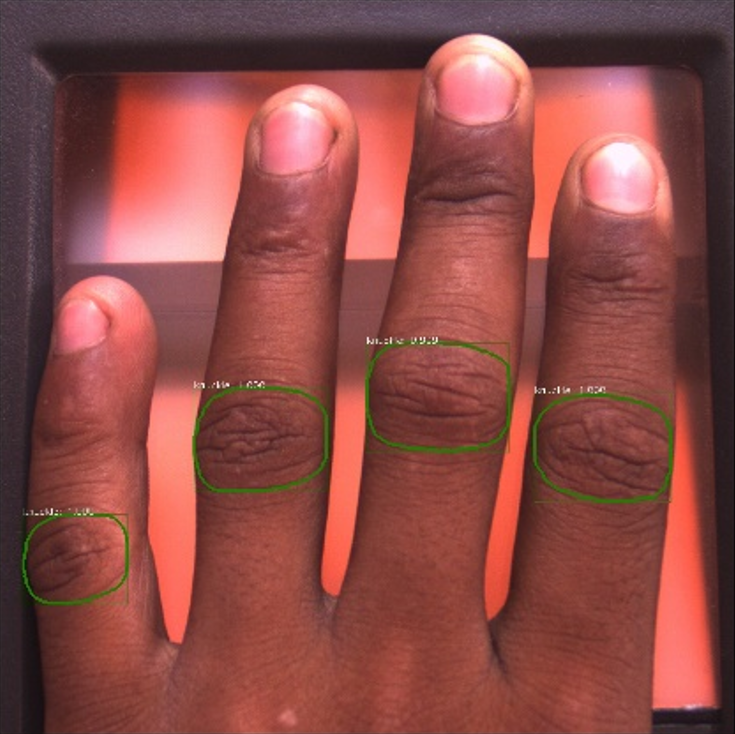
\includegraphics[width=1.105in]{Figures/4-4-2-a.png}%
    \label{4-4-2-a}}
    \subfloat[]{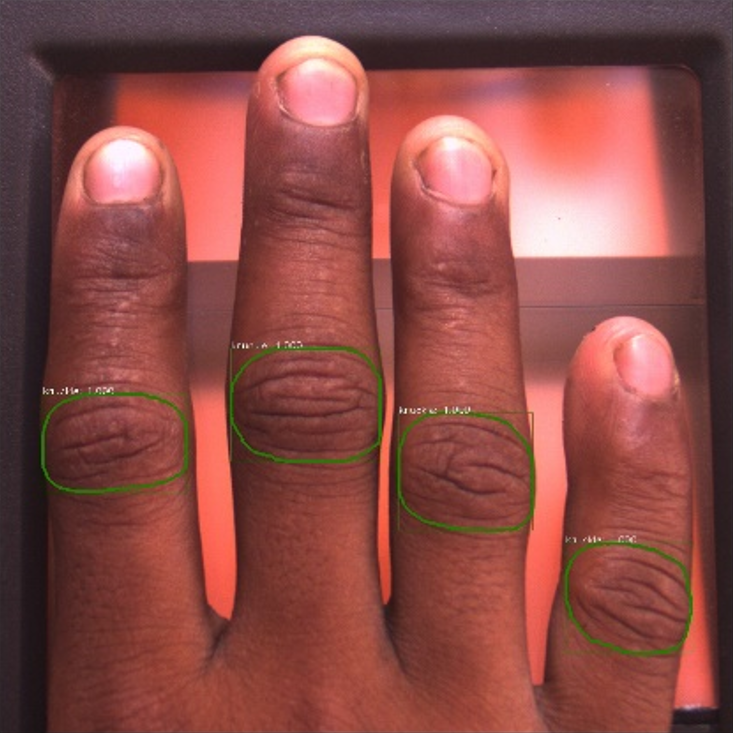
\includegraphics[width=1.105in]{Figures/4-4-2-b.png}%
    \label{}}
    \subfloat[]{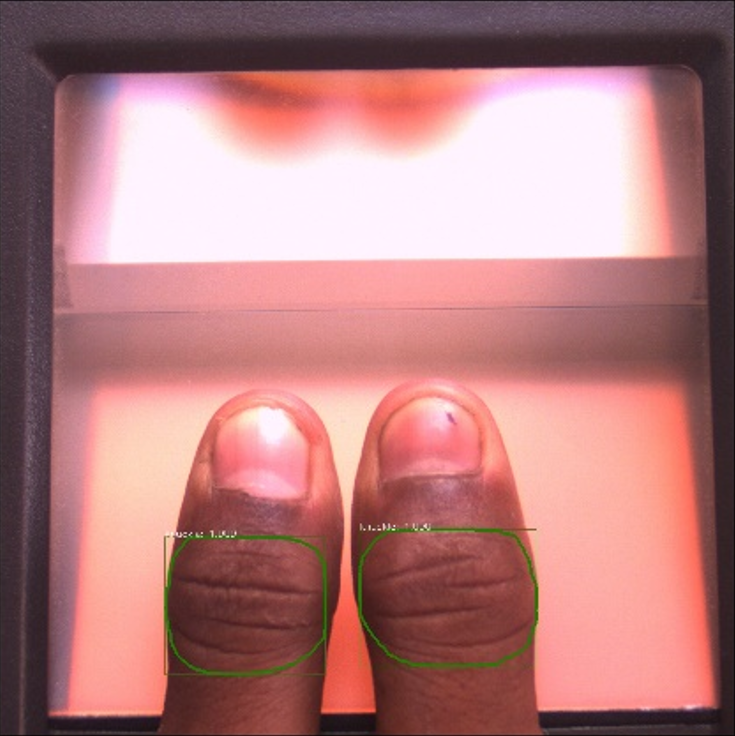
\includegraphics[width=1.1025in]{Figures/4-4-2-c.png} %
    \label{}}


    \subfloat[]{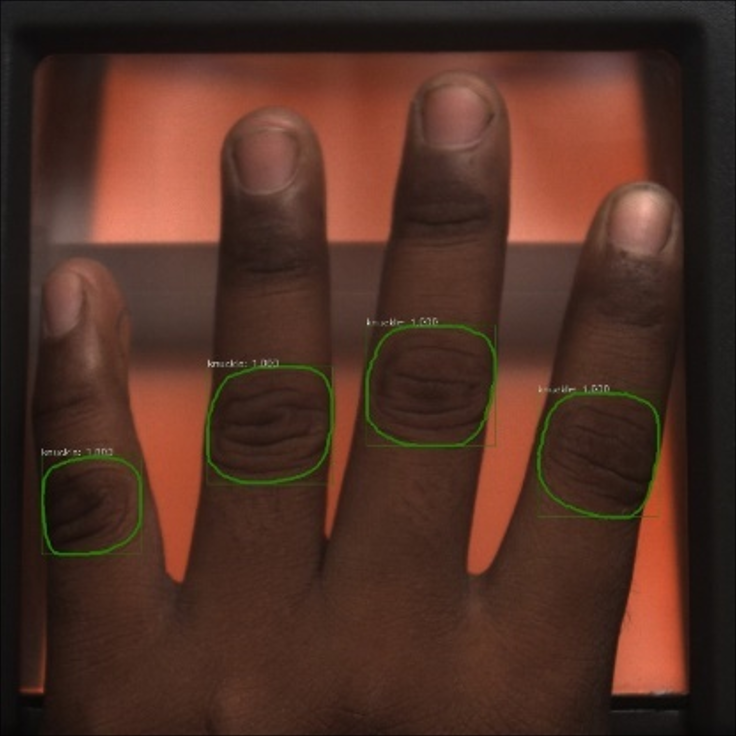
\includegraphics[width=1.1in]{Figures/4-4-2-d.png}%
    \label{}}
    \subfloat[]{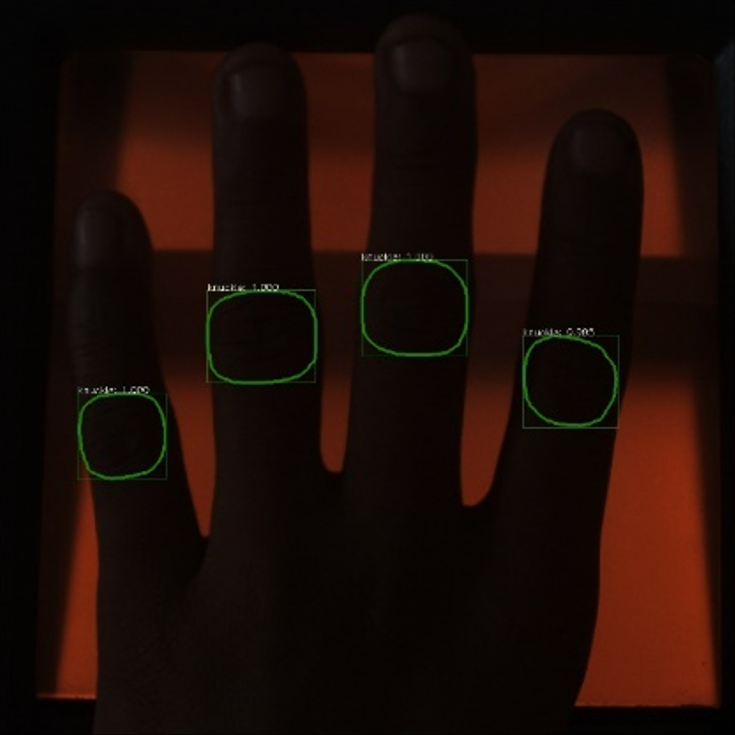
\includegraphics[width=1.1in]{Figures/4-4-2-e.png}%
    \label{}}
    \subfloat[]{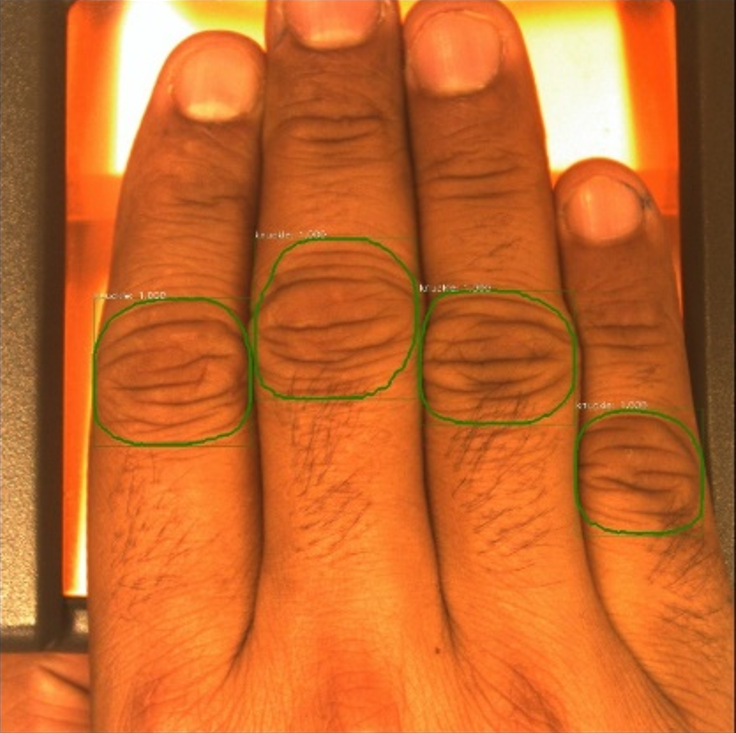
\includegraphics[width=1.105in]{Figures/4-4-2-f.png}%
    \label{}}
    \caption{Sample finger dorsal images acquired along with slap fingerprint images: (a)-(c) illustrates images from the same user using 4-4-2 imaging while (d)-(f) illustrates other users images acquired under the ambient imaging. These images also illustrate the knuckle region contours and respective bounding boxes in green color.}
    \label{capture-finger-knuckle}
    % \vspace{-0.4cm}
\end{figure}

\begin{figure}[!ht]
    \centering
    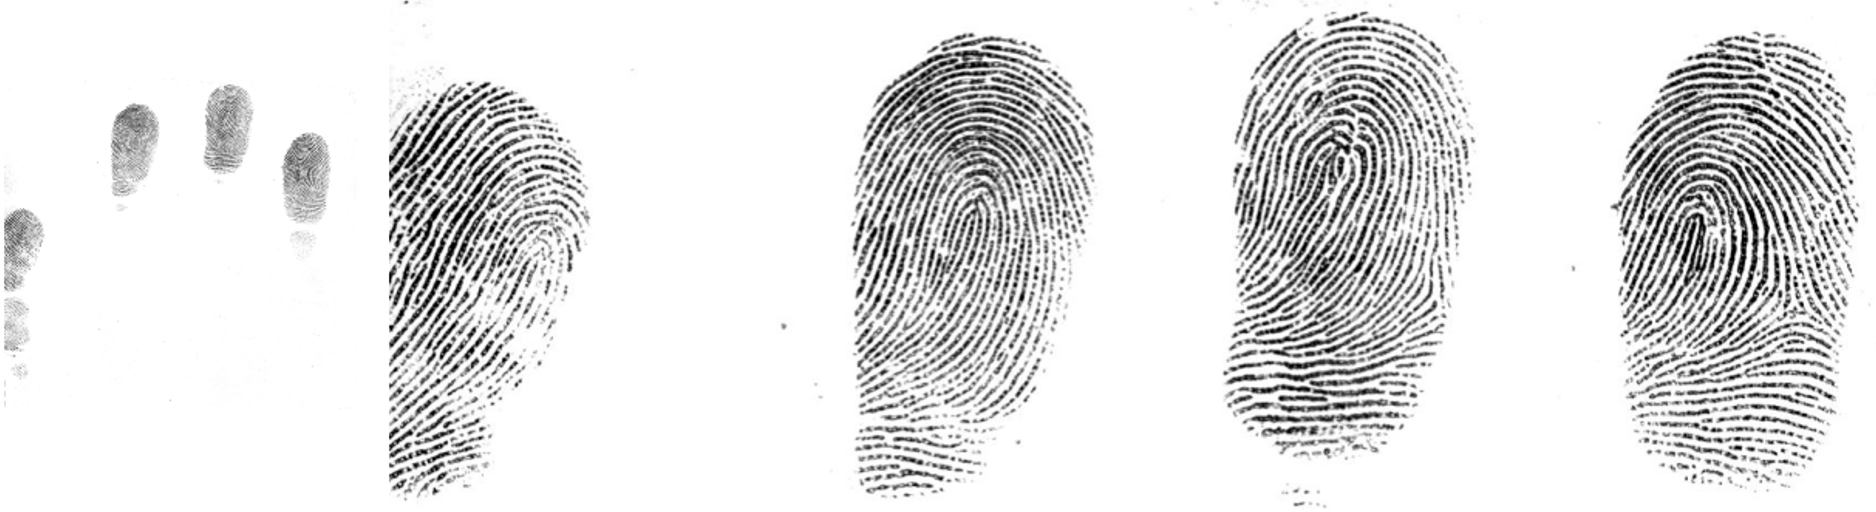
\includegraphics[width=3.4in]{Figures/4-4-2-fingerprint.png}
    \caption{Simultaneously acquired slap fingerprint image corresponding to the knuckle images shown in Fig. \ref{4-4-2-a}. Respective segmented fingerprint images are shown in (b)-(d).}
    \label{capture-finerprint}
\end{figure}

The block diagram for the finger-knuckle-assisted slap fingerprint identification system is shown in Figure 4. Acquisition of finger-dorsal surface images is synchronized with the slap-fingerprint image acquisition and therefore the two images are acquired using a single imaging shot. The finger knuckle images are acquired under ambient illumination, which inherently presents complex background resulting from the slap-fingerprint sensor surface. Therefore these images are first subjected to preprocessing operations to normalize the illumination. The key task is to accurately localize, i.e., detect and segment, four (or two) finger knuckle regions from such simultaneously acquired images. Section 2.1.1 explains our approach to automatically segment desired finger-knuckle regions from the acquired images. Each   of   the   detected   knuckle   region   images  are  firstly normalized to ensure are  firstly normalized to ensure alignment among segmented knuckle regions from the successive images and the approach detailed in Section 2.1.2. Detected finger knuckle regions are subjected to the feature extraction steps, to generate respective templates. These templates are matched during the user authentication to generate the respective finger-knuckle match score. The segmentation of fingerprint images is relatively easier, or quite matured, and such segmentation algorithms are widely provided with commercial slap-fingerprint sensor. Each of the segmented fingerprint images are subjected to the feature extraction to generate respective fingerprint templates. These templates are matched with the corresponding fingerprint templates, stored in the registration database, to generate respective fingerprint match score during the user authentication. Two simultaneously generated match scores, from the fingerprint and respective finger-knuckle images, are subjected to a dynamic fusion algorithm (as detailed in Section 3) to generate a consolidated match score for the user authentication.   


\begin{figure*}[!ht]
    \centering
    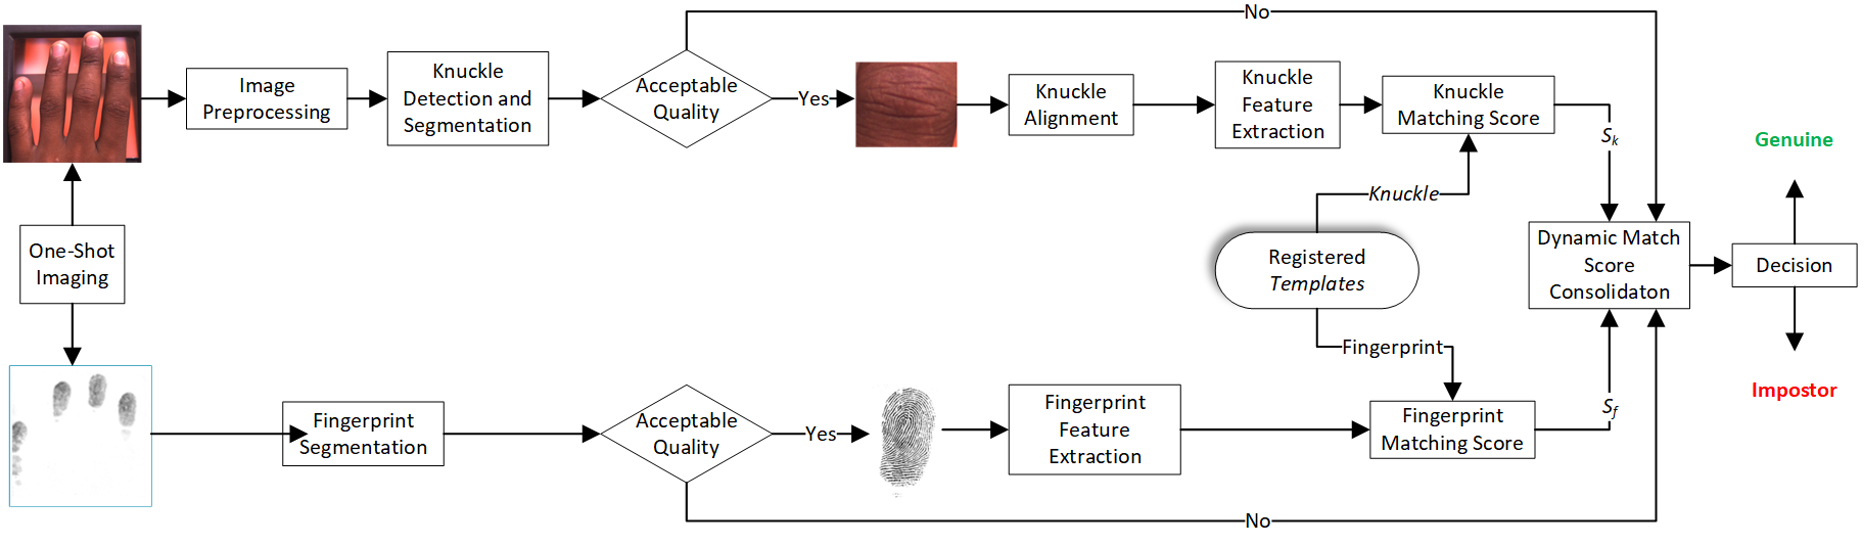
\includegraphics[width=7in]{Figures/block-diagram.png}
    \caption{Block diagram for the developed finger-knuckle assisted fingerprint identification system.}
    \label{block-diagram}
\end{figure*}

\subsection{Finger Knuckle Segmentation from Single-Shot Images}
\subsubsection{FINGER KNUCKLE DETECTION FROM MULTIPLE FINGERS}


\begin{figure}[!ht]
    \centering
    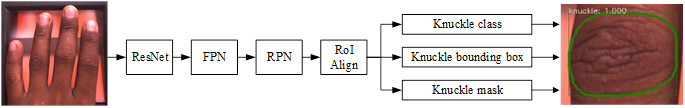
\includegraphics[width=3.5in]{Figures/mask-rcnn.png}
    \caption{Detecting multiple finger knuckle regions using a mask R-CNN based framework.}
    \label{mask-rcnn}
\end{figure}


Each of the simultaneously acquired, i.e. single-shot images during 4-4-2 imaging, knuckle images present multiple finger dorsal surfaces. Finger knuckle detectors introduced in the literature [7] are designed for images under uniform background and/or for the single finger dorsal surfaces. However the slap-fingerprint finger dorsal surface images present multiple fingers, which may be in full contact (see sample in Figure 2f) with each other and acquired under complex background with ambient illumination. Therefore finger-knuckle detectors employed in earlier research [6] can-not be employed to address our detection task. We, therefore, developed a \textit{specialized} mask R-CNN [15] based finger-knuckle detector for our system. The mask R-CNN [15] has shown its superior performance in object detection and segmentation tasks, for example we can observe impressive results for the COCO object detection and segmentation competition. Therefore, we developed a finger knuckle detector using the mask R-CNN framework as shown in Figure 5. Finger Knuckle images are fed into a standard CNN network (we use ResNet [30] here) and a Feature Pyramid Network (FPN) [11] to build multi-scale RoI features. From RoI features, Region Proposal Network (RPN) generates finger knuckle region proposals, which will be processed by RoI Align to further improve finger knuckle localization. Mask R-CNN generates three outputs: finger knuckle class label, finger knuckle bounding box, and finger knuckle segmentation mask. The finger knuckle detector training samples were collected from a separate subject whose images are not included in the finger-knuckle and fingerprint database. Since knuckle detection is not a complex task, we used ResNet-50 FPN as the backbone instead of ResNet-101 FPN. We used data augmentation [27], such as random rescaling, horizontal flipping and color jittering, to augment the training data. We also used contrast enhancement, during the preprocessing stage, to normalize the acquired images that are acquired under varying illumination.  

The mask R-CNN generates several bounding boxes that may or may not contain finger knuckle and therefore. The reason is that the bounding box may indicate \textit{minor} finger knuckle, or region that may look similar to the finger knuckle. In this work we only consider the \textit{major} finger knuckle as the region of interest, i.e., in rest of this pa-per the term finger knuckle refers to the \textit{major} finger knuckle. The bounding boxes that are generated by Mask R-CNN indicate possible locations of finger knuckles, and bounding boxes with higher confidence scores most likely the regions with correct localizations of the finger knuckle regions. Therefore, to identify the correct bounding box with the finger knuckle regions, we firstly assume that the bounding box with high confidence scores are more likely to indicate the finger knuckle. Secondly, the bounding box with high confidence score may still indicate incorrect location of finger knuckle. Therefore, we propose to incorporate the domain knowledge, i.e. relative geometric locations of the finger knuckle regions, to improve the finger knuckle detection capability. For the human finger knuckles, four finger knuckles on the acquired images are expected to be in a relative sequence along the horizontal or x-axis. Along the vertical or y-axis, middle finger knuckle and ring finger knuckle are expected to be higher than the index finger knuckle and ring finger knuckle. Finally, along the vertical axis, all four knuckles are not expected to be far away from each other.

\begin{figure}[ht!]
    \centering
    \subfloat[]{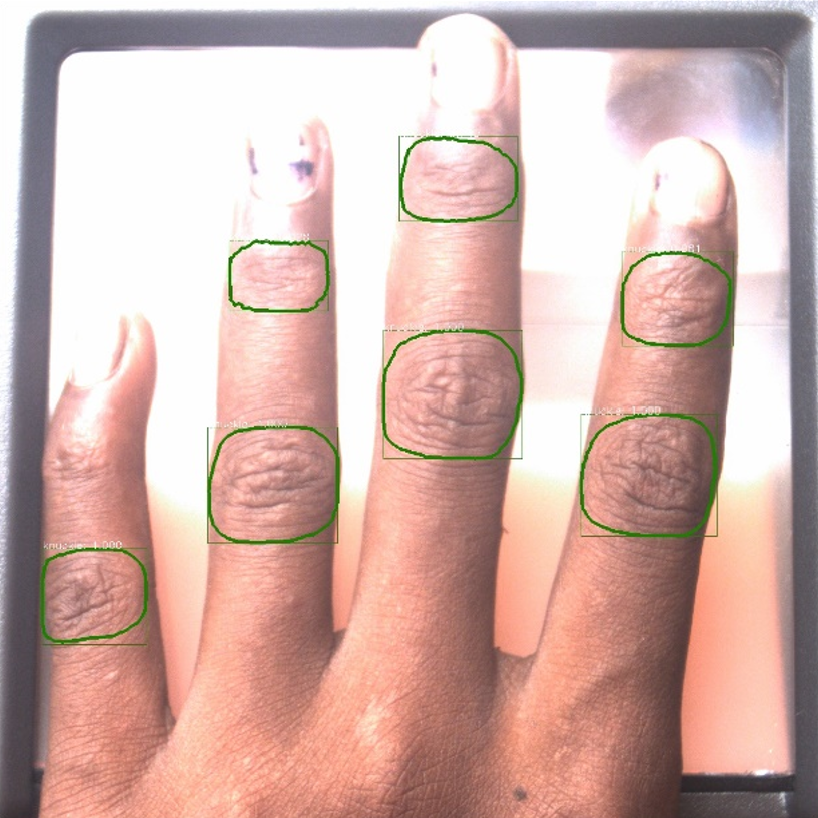
\includegraphics[width=1.6in]{Figures/select-before.png}%
    \label{}}
    \subfloat[]{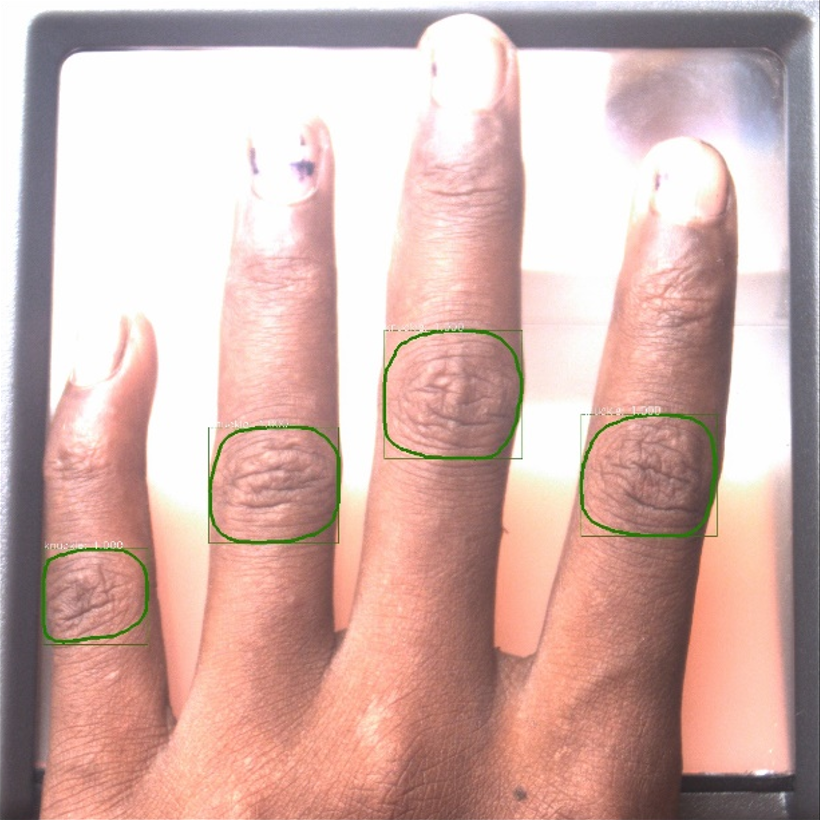
\includegraphics[width=1.6in]{Figures/select-after.png}%
    \label{}}

    \caption{The image on the left shows bounding boxes that are generated by a pre-trained Mask R-CNN model. The image on the right shows bounding boxes left after post-processing. The bounding boxes that do not include region of interest are excluded.}
    \label{select-finger-knuckle}
    % \vspace{-0.4cm}
\end{figure}

\begin{algorithm}[h!]
    \renewcommand{\algorithmicrequire}{\textbf{Input:}}
    \renewcommand{\algorithmicensure}{\textbf{Output:}}
    \caption{Post-processing for detected knuckle regions (bounding boxes)}
    \begin{algorithmic}[1]
        \REQUIRE Slap finger knuckle image $\bm{IMG}$, pre-trained Mask R-CNN model \\ 
        \ENSURE Finger knuckle set $\bm{KnuckleB = \{b_i\}_{i=1}^n, n\leq 4}$\\
        \STATE Generate the set of bounding boxes $B= \{b_i\}_{i=1}^m,m\geq n$ from $IMG$;
        \STATE If $m \leq 4$, then go to Step 14;
        \STATE Sort confidence score $s_i$ of each $b_i \in B, i = 1, ..., m$;
        \STATE Make a new set $candidateB= \{b_i\}_(i=1)^4$ where $s_i$ of each $b_i$ is the top four highest;
        \STATE For each $b_i \in candidateB, i=1,2,3,4$, remove $b_i$ from set $B$;
        \STATE Sort $b_i$ along x-axis from left to right;
        \STATE Denote $b_i$ from left to right as $b_1^{'}$, $b_2^{'}$, $b_3^{'}$,and $b_4^{'}$, and keep the original index of each $b_i$;
        \STATE For $b_i^{'}=(x_i,y_i)$, compute the following variables:\\
        \footnotesize{
            \begin{equation}
                \begin{aligned}
                    y_{min}=\min (y_1, y_2, y_3, y_4), y_{max}= \max (y_1, y_2, y_3, y_4)
                \end{aligned}
                \label{equation-1}
            \end{equation}
            \begin{equation}
                \begin{aligned}
                    disy = y_{max} - y_{min}, avg\_14=(y_1+y_4)/2
                \end{aligned}
                \label{equation-2}
            \end{equation}
            \begin{equation}
                \begin{aligned}
                    disy\_2\_14 = \left|y_1-avg\_14\right|, disy\_3\_14=\left|y_3-avg\_14\right|
                \end{aligned}
                \label{equation-3}
            \end{equation}
            \begin{equation}
                \begin{aligned}
                    disy\_14 = \left|y_1-y_4\right|, disy\_23=\left|y_2-y_3\right|
                \end{aligned}
                \label{equation-4}
            \end{equation}
            \begin{equation}
                \begin{aligned}
                    disy_l = \left|y_2-y_1\right|, disy_r=\left|y_4-y_3\right|
                \end{aligned}
                \label{equation-5}
            \end{equation}
            \begin{equation}
                \begin{aligned}
                    disx_l = \left|x_2-x_1\right|, disx_r=\left|x_4-x_3\right|
                \end{aligned}
                \label{equation-6}
            \end{equation}}
        \vspace{-0.2in}
        \STATE Check the following constraints:\\
        \footnotesize{
        Constraint (1): if $disy\_2\_14 \ge \tau_1 \times disy\_3\_14$ and $disy\_23 \ge \tau_1 \times disy\_14$ and $disy \ge \tau_2$, then $b_2^{'}$ is invalid, go to Step 11;\\
        Constraint (2): if $disy\_3\_14 \ge  \tau_1 \times disy\_2\_14$ and $disy\_23 \ge \tau_1 \times disy\_14$ and $disy \ge \tau_2$, then $b_3^{'}$ is invalid, go to Step 11;\\
        Constraint (3): if $disy_l \ge \tau_3$ and $disx_l \le \tau_4$, then $b_1^{'}$ is invalid, go to Step 11;\\
        Constraint (4): if $disy_r \ge \tau_3$ and $disx_r \le \tau_4$, then $b_4^{'}$ is invalid, go to Step 11;\\
        Constraint (5): if $y_1 \times \tau_5 \le y_2$, then $b_1^{'}$ is invalid, go to Step 11;\\
        Constraint (6): if $y_4 \times \tau_5 \le y_3$, then $b_4^{'}$ is invalid, go to Step 11;}
        \STATE If all conditions in Step 9 are satisfied, then go to Step 14;
        \STATE For invalid bounding box $b_i^{'}$, find the corresponding bounding box $b_i$ that is kept in Step 6, remove $b_i$ from $candidateB$;
        \STATE If $B = \emptyset$, then go to Step 14;
        \STATE Find $b_i \in B$ whose $s_i$ is the highest, add $b_i$ to $candidateB$, remove $b_i$ from $B$. Go to Step 6;
        \STATE $KnuckleB \gets candidateB$

    \end{algorithmic}
\end{algorithm}

We designed an algorithm to automatically determine the four bounding boxes or the regions of our interest. This algorithm can be summarized as follows: firstly, we choose four bounding boxes with the top four highest confidence score and check if they are compliant with their expected geometrical distribution. In absence of such compliance, we automatically remove the incorrect bounding box, from the rest or the shortlisted bounding boxes, choose the one with the highest confidence score. As shown in Algorithm 1, we repeat this process until all the bounding boxes, or the chosen regions, are compliant with their expected geometrical distribution.

\begin{figure}[!ht]
    \centering
    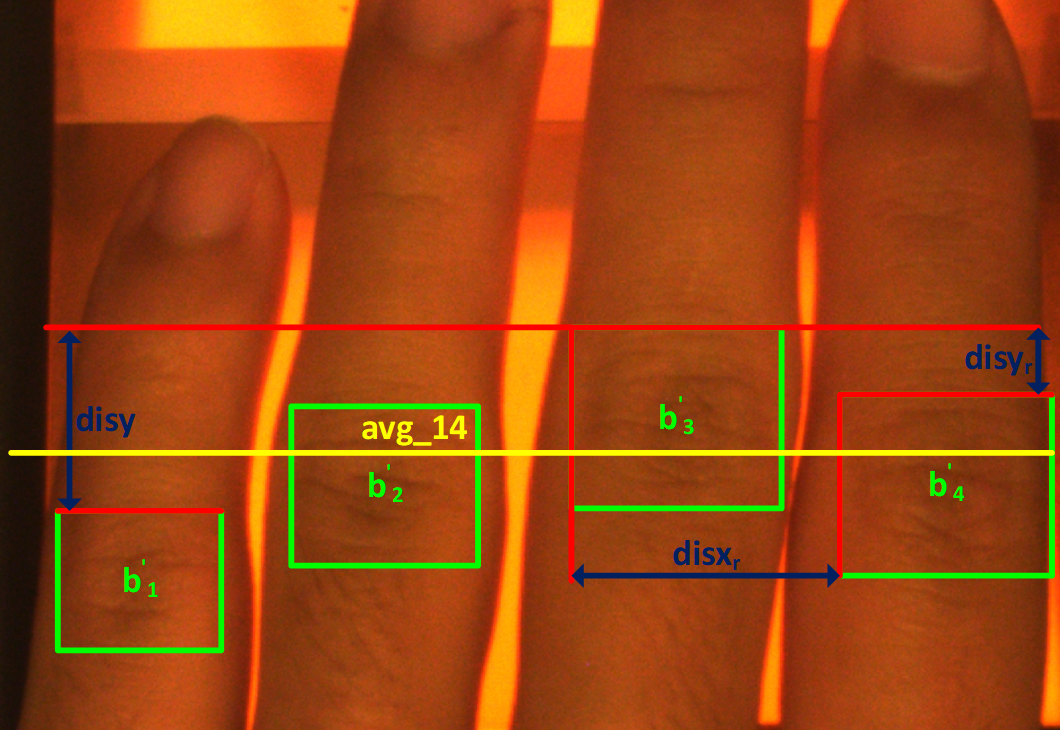
\includegraphics[width=2.5in]{Figures/select-algorithm.png}
    \caption{Illustration for the variables that are defined in Algorithm 1. $b_1^{'}$, $b_2^{'}$, $b_3^{'}$, and $b_4^{'}$ (in green) are bounding boxes that have been sorted along x-axis. \textit{disy} (in blue) and \textit{avg\_14} (in yellow) are variables in equation (2). $disy_r$ and $disx_r$ are variables in equation (5) and (6).}
    \label{select-algorithm}
\end{figure}


The Algorithm 1 can be briefly explained as follows. Step 1 firstly generates the set of all bounding boxes $b_i$ (Figure 6) that may include finger knuckle like patterns. Each bounding box $b_i$ is represented by top-left coordinate $(x_{1i},y_{1i})$, bottom-right coordinate $(x_{2i},y_{2i})$, and a corresponding confidence score $s_i$ ranging from 0 to 1. Step 2 to Step 6 selects bounding boxes with the \textit{highest} confidence scores and sort them along horizontal axis. In step 8, for simplicity reason, the top-left coordinate of each bounding box is represented by $(x_i,y_i)$, $i=1,2,3,4$, because only top-left coordinate is required for the later use. Also, for the reasons of simplicity, the top-left coordinate is used to identify the location of each of the bounding boxes. The coordinate of each bounding box is normalized with respect to the width and height of the image. For normalization, given the height and the width of the image, the vertical and horizontal coordinate of the bounding box is normalized by the height or the width respectively. The variables that are computed from step 8 are used to control the geometrical distribution of the four bounding boxes so that they are compliant with the expected geometrical distribution of four knuckles. The variable $disy$ in equation (2) is computed to ensure that along the vertical axis two locations, i.e. the bounding box on the top and at the bottom, are not far away from the other bounding boxes. The variables $disy\_2\_14$, $disy\_3\_14$, $disy\_23$ and $disy\_14$ in equation (3)-(4) are similarly used to check the two knuckle locations in the middle (for slap finger image, the two knuckles correspond to middle knuckle and ring knuckle) so that these two knuckles are closer to each other. These are guaranteed by constraints in (1) and (2). Similarly, the constraints in (3)-(6) are used to check the validity of knuckle locations on both sides. The constraints in (3) and (5) ensure that the appearing locations at the bounding box is valid for the left-most knuckle (the left-most knuckle correspond to little knuckle of left hand and index knuckle of right hand). Similarly, the constraints in (4) and (6) are incorporated to ensure that the bounding box location is valid for the right-most knuckle (the right-most knuckle correspond to index knuckle of left hand and little knuckle of the right hand). The parameter $disx_l$ and $disx_r$ in equation (6) are used to discard the possibility that the two bounding boxes are located or detected on the one/same finger. The hyperparameters in Step 9 are empirically selected and for all our experiments in this paper we fixed $\tau_1=1.2$, $\tau_2=0.23$, $\tau_3=0.25$, $\tau_4=0.05$, and $\tau_5=1.02$.

\subsubsection{Finger knuckle alignment and normalization}

As can be seen from a sample slap-fingerprint dorsal image in Figure 2 that the presented fingers from the users may not be strictly upright, and the extent of such finger knuckle orientation can vary for different fingers even in the \textit{same} image. Therefore, the orientation of finger-knuckle regions also varies for each of the fingers. In absence of any orientation normalization, the match accuracy between different knuckle images can significantly degrade. We therefore automatically estimate the orientation for each of the fingers present in the acquired image and incorporate alignment in the segmented or normalized finger knuckle images.

\begin{figure}
    \centering
    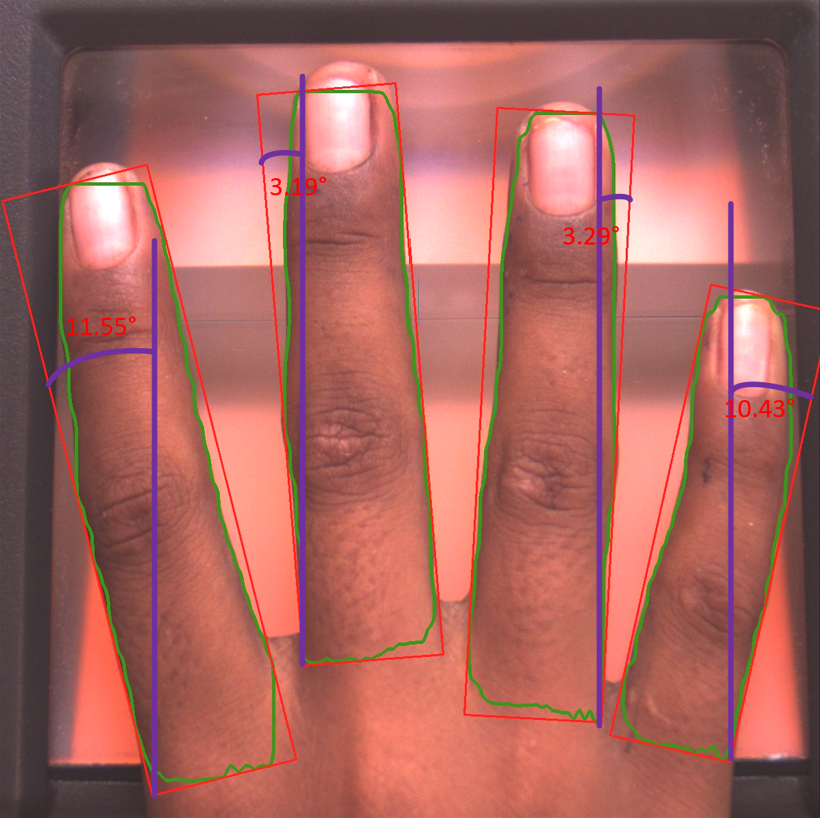
\includegraphics[width=2.5in]{Figures/finger-orientation.png}
    \caption{The bounding box in red and contour in green indicate the detection and segmentation of respective fingers. The vertical line and curve in purple, which are \textit{manually} drawn, indicate the orientation of each finger. The number in red color near the purple curve indicates the estimated orientation of respective finger.}
    \label{finger-orientation}
\end{figure}

The orientation of finger knuckle region is inherently linked with the orientation of the fingers presented on the slap-fingerprint sensor. Therefore, a trained Mask R-CNN is used to detect the fingers. Based on the segmented finger area from this finger detector, a rotated rectangular bounding box with minimum area is fitted. The orientation of the largest side of this rectangle indicates the orientation of the respective finger. Figure 8 illustrates a sample image and such estimated orientation for each of the fingers in this image. The orientation of each of the fingers is used to automatically segment the aligned or normalized finger knuckle images for the feature extraction. Figure 9 illustrates the effectiveness of such orientation alignment where the segmented images without alignment and respective images after alignment are shown from a sample image in our database. Table 1 presents a summary of estimated orientation for each of the fingers for the images in our database. It can be observed that the orientation of each finger knuckle region varies, and the average orientations of the same finger knuckle, from the left hand and the right hand, are quite close to each other.

\begin{figure}
    \centering
    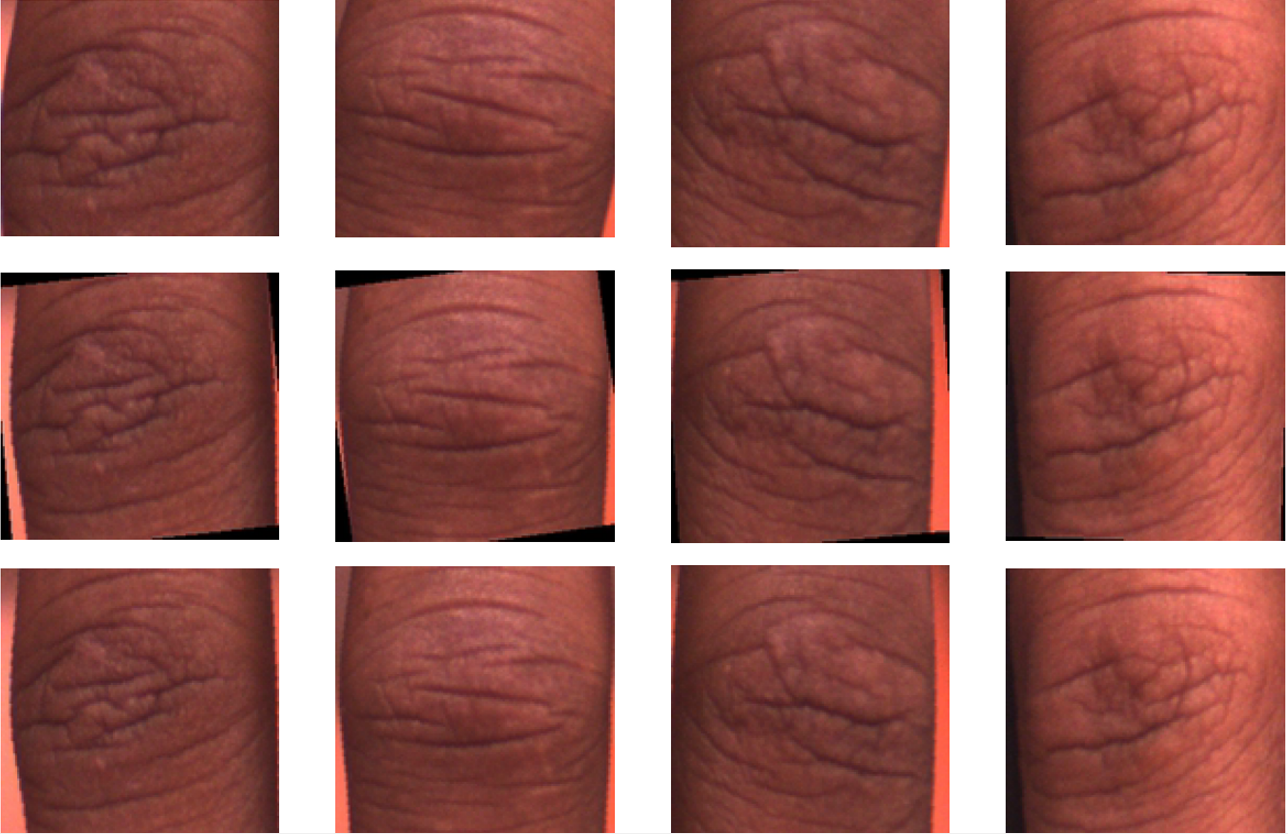
\includegraphics[width=2.7in]{Figures/orientation-normization.png}
    \caption{Segmented finger knuckles images from a sample slap-fingerprint dorsal image. First row illustrates segmented knuckle image \textit{without} orientation normalization while last row \textit{with} and without rotation. The rotated images are shown in the middle row, to illustrate the extent of orientation correction for the respective images in the first row.}
    \label{orientaion-normlization}
\end{figure}


\begin{table}[]
    \caption{Summary of the estimated orientation (in degrees) for different knuckle in our databases.}
    \scalebox{0.9}[1]{
    \begin{tabular}{cccccccc}
    \hline
    Finger      & min  & max   & mean & Finger       & min  & max   & mean \\ \hline
    left thumb  & 0.00 & 29.24 & 7.00 & right thumb  & 0.00 & 26.97 & 6.21 \\
    left index  & 0.02 & 19.49 & 6.34 & right index  & 0.05 & 20.30 & 6.11 \\
    left middle & 0.01 & 13.34 & 3.47 & right middle & 0.00 & 20.96 & 3.56 \\
    left ring   & 0.01 & 14.67 & 3.18 & right ring   & 0.00 & 12.11 & 3.13 \\
    left little & 0.00 & 19.31 & 4.41 & right little & 0.02 & 17.77 & 4.28 \\ \hline
    \end{tabular}}
    \label{summary-orientation}
\end{table}
